% Created 2023-01-24 Tue 10:40
\documentclass[9pt, b5paper]{article}
\usepackage{xeCJK}
\usepackage{minted}
\usepackage[T1]{fontenc}
\usepackage[scaled]{beraserif}
\usepackage[scaled]{berasans}
\usepackage[scaled]{beramono}
\usepackage{graphicx}
\usepackage{xcolor}
\usepackage{multirow}
\usepackage{multicol}
\usepackage{float}
\usepackage{textcomp}
\usepackage{algorithm}
\usepackage{algorithmic}
\usepackage{latexsym}
\usepackage{natbib}
\usepackage{geometry}
\geometry{left=1.2cm,right=1.2cm,top=1.5cm,bottom=1.2cm}
\newminted{common-lisp}{fontsize=\footnotesize} 
\usepackage[xetex,colorlinks=true,CJKbookmarks=true,linkcolor=blue,urlcolor=blue,menucolor=blue]{hyperref}
\author{deepwaterooo}
\date{\today}
\title{unity游戏热更新服务端服务器}
\hypersetup{
  pdfkeywords={},
  pdfsubject={},
  pdfcreator={Emacs 27.2 (Org mode 8.2.7c)}}
\begin{document}

\maketitle
\tableofcontents


\section{笔记}
\label{sec-1}
\section{综述}
\label{sec-2}
\begin{itemize}
\item 这个框架相对比较平民化比较亲民,文档相对健全,关键模块和知识点讲解得相对透彻完善,更关键的是使用的人可能会比较多。自己遇到问题的时候能够网络上寻求的帮助来源多一点儿。会主要参考这个来搭写自己的框架
\end{itemize}

\section{帐户服 + 数据库 + 登录中心服 + 网关服: 具体设计逻辑相关实现源码学习}
\label{sec-3}
\begin{itemize}
\item 下面主要记录别人站在相对比较高的角度总结出来的架构:\url{https://blog.csdn.net/Q540670228/article/details/123592622}
\end{itemize}

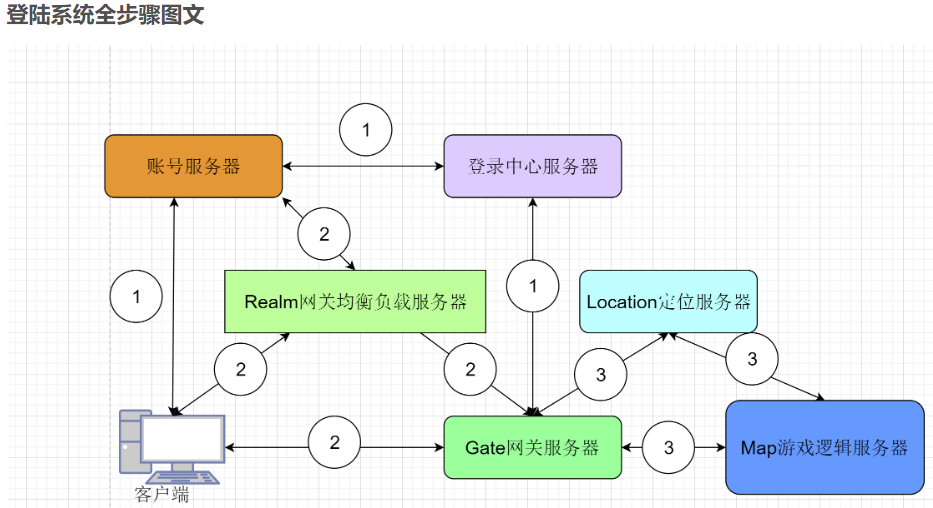
\includegraphics[width=.9\linewidth]{./pic/readme_20230124_102951.png}
\subsection{一. 账号登录}
\label{sec-3-1}
\subsubsection{1.客户端请求获取账户信息}
\label{sec-3-1-1}

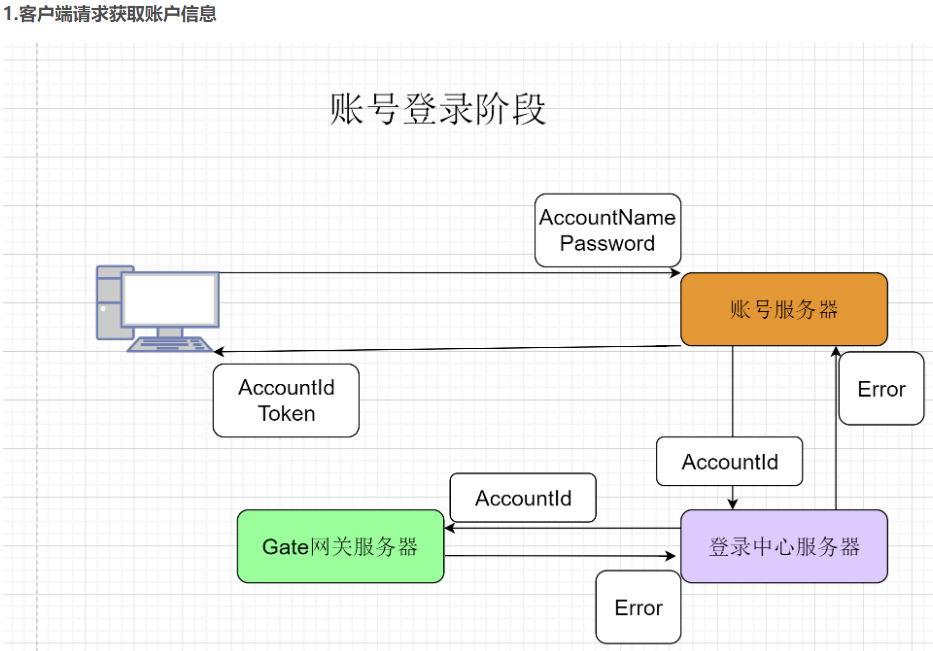
\includegraphics[width=.9\linewidth]{./pic/readme_20230124_103209.png}
\begin{itemize}
\item 客户端向账号服务器发送账户名和密码的消息,请求进行登录
\item 账号服务器和数据库交互,对信息进行验证或注册,获取账户唯一标识AccountId
\item 处理顶号逻辑,向登录中心服务器发送请求消息包含AccountId
\item 登录中心的组件存有AccountId和其所在区服zone的映射,若不存在AccountId直接返回即可
\item 若存在AccounId,根据其所在区服zone获取网关服务器的InstanceId,进而向其发送下线消息
\item 网关服务器存有所有客户端的映射实体Player(存有sessionInstanceId,UnitId,AccountId等)
\item 根据AccountId获取Player并通过Player的SessionInstanceId获取网关到客户端的session并释放
\item 为Player添加下线组件PlayerOfflineOutTimeComponent 后 返回即可
\item 登陆中心接到返回消息继续返回给账号服务器即可
\item 账号服务器处理完顶号逻辑后,自身也应缓存AccountId和自身的SessionId,做一次自身的顶号逻辑
\item 最后随机生成一个Token,把Token和AccountId发回给客户端
\item 客户端将AccountId Token等基本信息保存在zoneScene的AccountInfo组件中,供后续使用
\end{itemize}
\subsubsection{2. 客户端请求获取区服信息}
\label{sec-3-1-2}

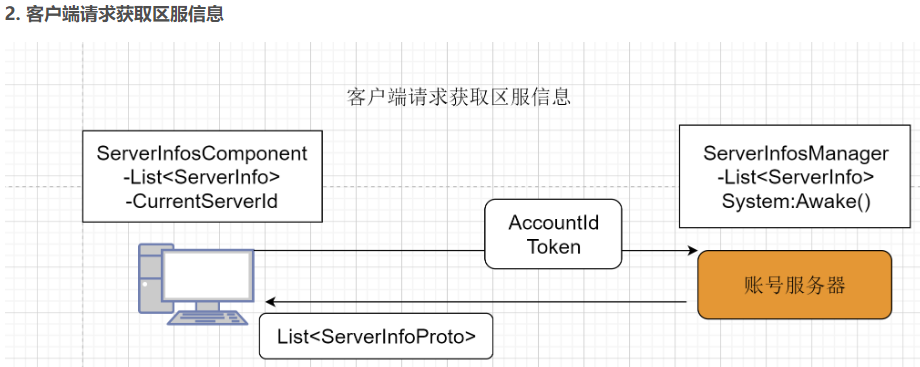
\includegraphics[width=.9\linewidth]{./pic/readme_20230124_103245.png}
\begin{itemize}
\item 定义ServerInfo区服信息实体(区服名,状态)及与proto映射的相互转换行为,并在双端均定义组件用以保存区服信息列表。
\item 服务器的组件要为其添加行为,Awake时就应该将数据库中的区服信息读取出来放入组件的信息列表中
\item 客户端向账号服务器发送信息,请求获取所有的区服信息,需要发送AccountId和Token用于验证账户
\item 账号服务器将服务器信息列表转换为其对应的ServerInfoProto列表,并发送回客户端
\item 客户端接收到后将proto转换回ServerInfo并保存到组件当中,显示到UI层供用户选择。
\item \textbf{注意 ServerInfoProto存在的意义,ET框架下网络传输的必须是Proto对象,不能直接是实体,所以需要定义Proto作为传输对象,在双端进行转换使用。}
\end{itemize}
\subsubsection{3. 客户端请求 获取/创建/删除 角色信息}
\label{sec-3-1-3}
\begin{enumerate}
\item 获取角色信息
\label{sec-3-1-3-1}

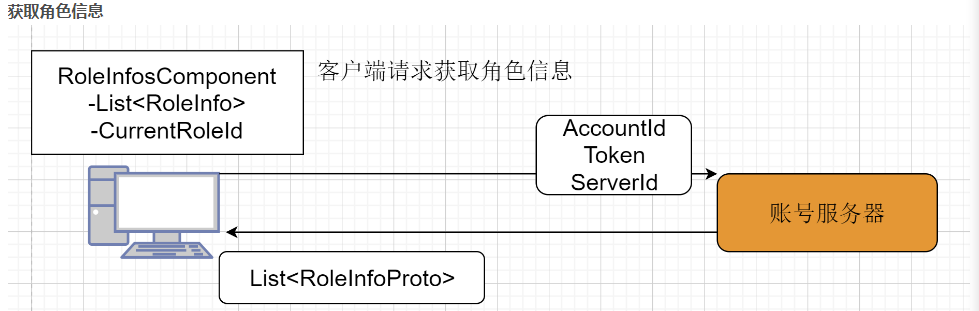
\includegraphics[width=.9\linewidth]{./pic/readme_20230124_103354.png}
\begin{itemize}
\item 获取角色信息的步骤和获取服务器信息很类似
\begin{itemize}
\item 定义RoleInfo实体(Name,AccountId,State,ServerId),并为其提供和proto的相互转换行为
\item 实体是双端可以公用的,但账号服务器无需保存,只需在请求时从数据库获取完发回即可
\item 客户端向服务器发送消息请求获取 当前账户在当前区服下的所有未冻结的角色
\item 服务器通过Id和Token验证身份后,从数据库中获取所有角色信息转换成proto对象发回客户端
\item 客户端收到后将proto转换成RoleInfo存储在相应的组件中,显示到UI层供用户选择。
\end{itemize}
\end{itemize}
\item 创建角色信息
\label{sec-3-1-3-2}

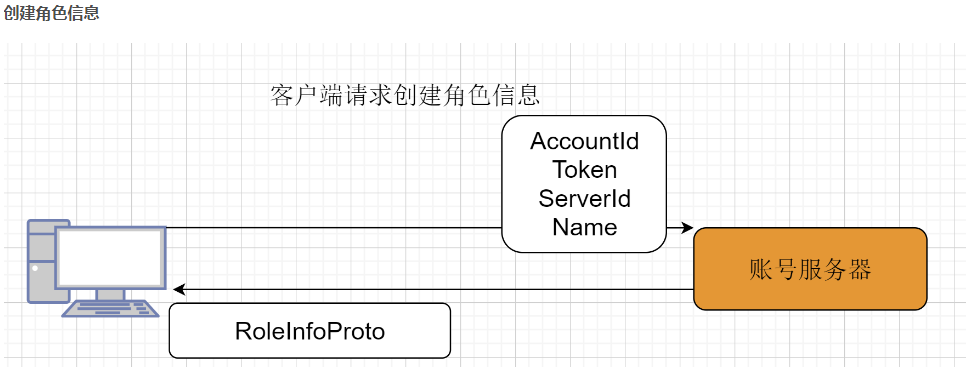
\includegraphics[width=.9\linewidth]{./pic/readme_20230124_103625.png}
\begin{itemize}
\item 用户和UI交互输入名称并点击按钮创建角色
\item 将用于验证的信息以及ServerId和用户输入的姓名一并发向服务器请求创建角色(区服间角色独立)
\item 服务器判断是否有重复角色,若没有则创建新角色RoleInfo,并对其各属性进行初始化。
\item 初始化利用Id创建使用GenerateUnitId,创建完成后保存到数据库中并转换成Proto发回客户端
\item 客户端收到RoleInfoProto后转换成RoleInfo并缓存起来,然后在UI管理处进行刷新UI循环列表
\end{itemize}
\item 删除角色信息
\label{sec-3-1-3-3}

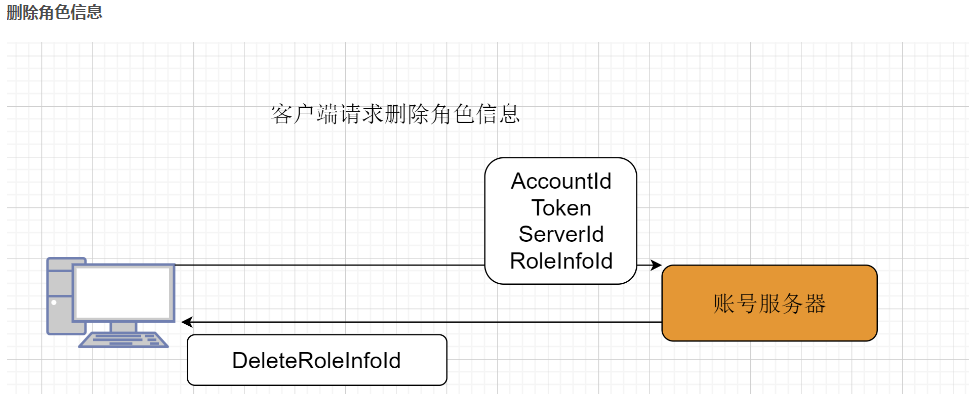
\includegraphics[width=.9\linewidth]{./pic/readme_20230124_103649.png}
\begin{itemize}
\item 在UI界面的循环列表为每个角色添加选择按钮,选择后会为组件的CurrentRoleId赋值选中的角色
\item 向账号服务器发送请求删除角色的信息,其中的RoleInfoId即为选择的CurrentRoleId。
\item 账号服务器在客户端中查询到指定Id的RoleInfo将其状态设置为Freeze冻结并修改名称(防止后续注册同名问题)
\item 发回客户端删除的RoleInfo的Id,客户端接收后在组件集合中将其移除并刷新UI界面。
\end{itemize}
\end{enumerate}
\subsection{二. 网关服务器的连接}
\label{sec-3-2}

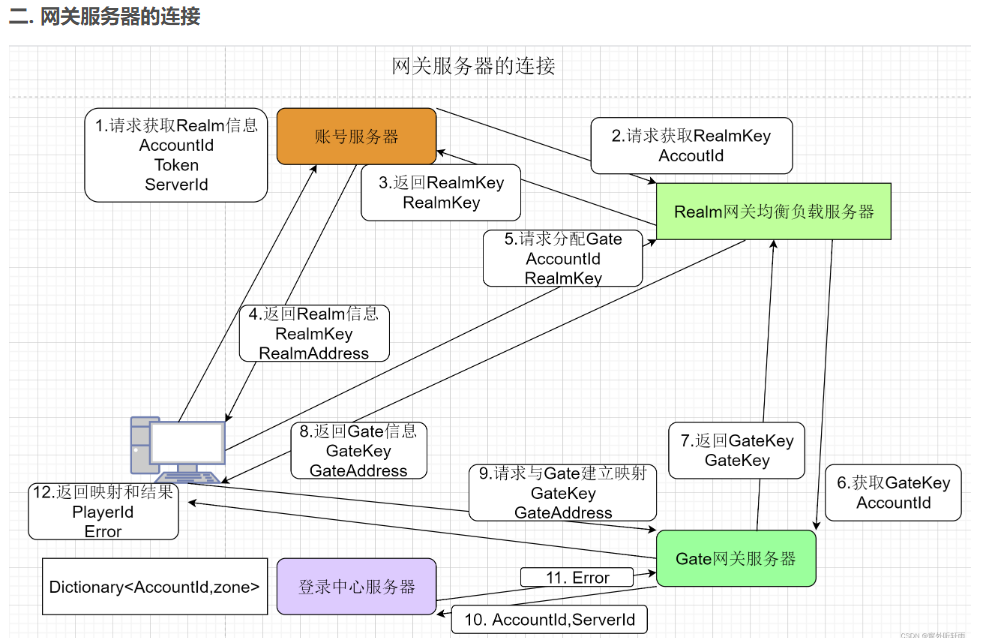
\includegraphics[width=.9\linewidth]{./pic/readme_20230124_103753.png}
\begin{itemize}
\item 网关服务器的的连接其实就是,客户端先和Realm网关连接请求其分配一个Gate网关,然后客户端去连接此Gate网关。
\end{itemize}
\subsubsection{1. 请求连接Realm网关}
\label{sec-3-2-1}
\begin{itemize}
\item 向账号服务器请求获取Realm网关的地址和令牌,需要区服Id,一般一个区服下有一个Realm
\item 账号服务器通过配置文件获取Realm网关的内网地址(sceneInstanceId),并向其请求获取RealmKey令牌。
\item Realm网关随机生成令牌RealmKey 和 AccountId将映射保存在组件中,将Key发回账号服务器
\item 账号服务器通过配置文件获取Realm网关的外网地址(OuterIPPort),和令牌RealmKey一并发回客户端
\end{itemize}
\subsubsection{2. 请求和Gate网关连接}
\label{sec-3-2-2}
\begin{itemize}
\item 客户端与账号服务器断连,与Realm建立连接,并向其请求分配网关服务器(即获取一个网关信息)
\item 一个区服下一般有多个Gate,Realm通过与账户Id取模的方式固定分配给此账户一个Gate,向此Gate请求获取GateKey
\item Gate网关服务器随机生成一个GateKey并将AccountId和GateKey的映射关系保存供后续验证,并发回Key
\item Realm服务器将Gate信息(key,address-配置文件得)发回客户端,客户端与Realm进行断开,准备连Gate
\end{itemize}
\subsubsection{3. 建立Gate映射对象Player}
\label{sec-3-2-3}
\begin{itemize}
\item 客户端一般会与Gate长时间连线,需要为Session添加心跳组件PingComponent,请求在Gate中创建映射对象Player
\item 步骤10 和 步骤11,主要是客户端与Gate建立连接后,将账户Id和区服号发送至登陆中心服务器进行注册添加,登录逻辑中会通过此服务器的记录进行顶号逻辑,通过区服号和AccountId利用Realm帮助类能唯一确定Gate,再给Gate发送下线消息即可。
\end{itemize}
\subsubsection{建立Player步骤}
\label{sec-3-2-4}
\begin{itemize}
\item 建立Player实体(AccountId,UnitId,SessionInstanceId,state),Player和账户ID,网关和客户端的Session连接以及Unit达到一一对应
\item 为网关到客户端的Session添加PlayerComponent保存所有Player实体(AccountId和Player映射字典),并为其添加SessionStateComponent,用于判断网关连接是否处于Normal或Game(便于后续Unit逻辑)
\item 为网关到客户端Session添加SessionPlayerComponent组件(AccountId,PlayerInstanceId)和Player一一对应,即在网关连接Session的此组件上直接获取相应Player,这样处理后续的游戏逻辑就不用每次都发送AccountId从PlayerComponent中获取了(节省传输量)
\item 判断是否可以复用Player,顶号下线时可以复用(后面有流程图解释),如果复用必须移除Player身上的下线组件,更新Session,即更新Player身上的SessionInstanceId和Session身上的SessionPlayerComponent重新创建。
\item 如果不是顶号等操作,直接创建Player并初始化即可,PlayerId用RoleId,UnitId暂时用RoleId,后续创建出游戏逻辑服Unit后用其替换。
\end{itemize}
将PlayerId返回给客户端供客户端可能使用。
\subsection{三. 游戏逻辑服务器连接}
\label{sec-3-3}
-​ 游戏逻辑服务器的连接本质上并不是客户端和其直接相连,而是通过在游戏服务器上建立一个映射对象和客户端绑定,客户端以后即可通过此映射对象的Id,通过网关转发和Location服务器的定位,将消息发送到服务器下的映射对象中。

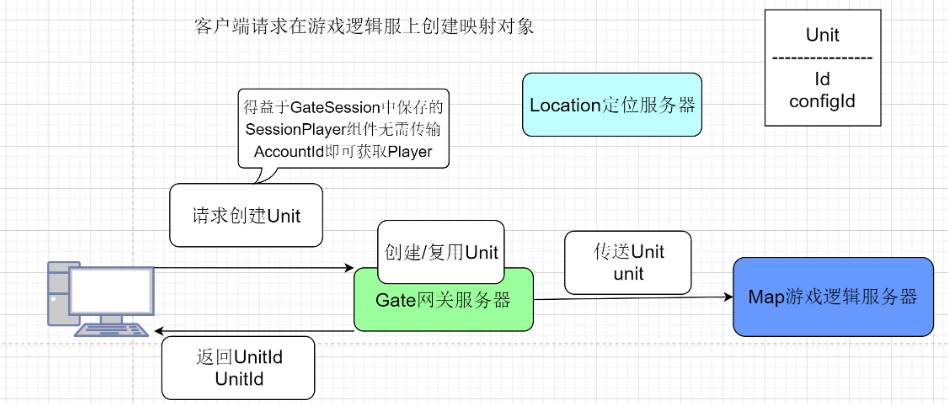
\includegraphics[width=.9\linewidth]{./pic/readme_20230124_103930.png}
\begin{itemize}
\item 客户端向Gate网关请求在Map服务器上创建Unit映射对象
\item 网关服务器先判断是否是顶号操作(利用Player的状态并向Player的Unit发送测试消息),验证成功后可以直接复用Player下的Unit并将UnitId返回客户端。
\item 若非顶号,则需要先临时为Player添加gateMapComponent组件,其下有一个属性Scene,在此Scene中创建一个Map场景用于后续传送Unit,(TransferHelper只能用于Map场景的传送,所以才做这一步)
\item 在上述创建的Map场景下创建Unit对象,UnitId可直接使用Player的Id即RoleId,然后必须为Unit添加UnitGateComponent,其中保存了gateSessionActorId即gateSessionInstanceId,(这样就可以利用Unit直接给客户端下发消息了)。
\item 利用配置文件获取Map服务器地址,利用TransferHelper的Transfer函数将unit传送到Map游戏逻辑服务器中
\item Transfer传送实现机制,实现以下机制后返回消息
\begin{itemize}
\item 通知客户端切换场景(直接利用unit下组件中gateSessionInstanceId直接下发即可)
\item request消息中保存Unit并将Unit下所有实现了ITransfer接口的组件保存起来一会一起传输过去
\item 删除当前Unit下的MailBoxComponent让发给此Unit的消息重发到正确位置(可能Unit还没传输过去就有信息发过来了)
\item 对Location定位服务器进行加锁,发送IActor消息传输给Map服务器,并释放当前Unit
\item Map服务器接收到消息将Unit和其组件重新添加(AddChild)到在此服务器下的UnitComponent中,将Unit添加到此组件集合中(传输时无法传输原Unit对象下的组件,只能将原Unit下基础属性以proto传递过来,在此还需重新生成)
\item 向客户端发相应的消息和属性,让客户端同步显示出角色并将Unit实体加入AOIEntity(AOI作用笔者暂且还未研究大概跟客户端有联系)
\end{itemize}
\item 传送完毕后将UnitId传回客户端即可,后续客户端就可利用UnitId发送IActorLocation消息和服务器上的Unit发送消息了。
\end{itemize}
\subsection{四. 顶号逻辑流程图}
\label{sec-3-4}

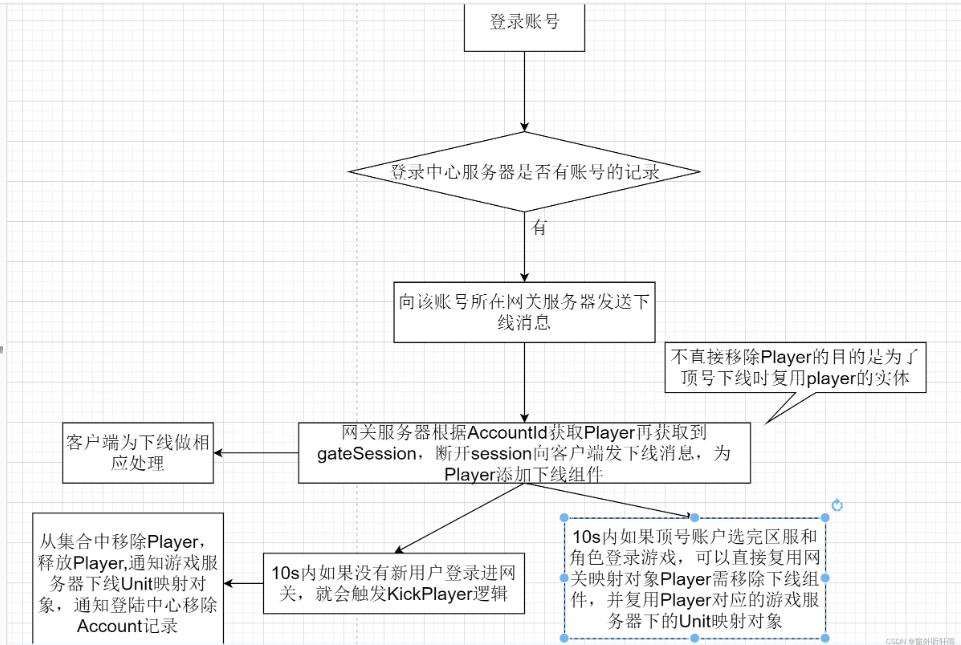
\includegraphics[width=.9\linewidth]{./pic/readme_20230124_104006.png}
\begin{itemize}
\item ​顶号逻辑属于是账号系统较为复杂的逻辑,其主要用到了中心登录服务器暂存玩家当前状态,并创建了Player和Unit映射对象,通过Player暂存到网关中实现顶号逻辑 可以无需重新创建Player和Unit直接更新属性复用,大大提高了顶号的效率。
\end{itemize}
% Emacs 27.2 (Org mode 8.2.7c)
\end{document}